\documentclass[12pt]{article}
\usepackage[utf8]{inputenc}
\usepackage{tikz}

\title{Readme project1 compilers}
\author{Emmanuel Rosales y Ernesto Lang }
\date{March 2016}

\begin{document}
\title{
		\begin{huge}
		Instituto Tecnol\'ogico de Costa Rica.
	   \end{huge}
	   \newline
	   \begin{Large}
	   \\Compiladores e Int\'erpretes
	   \\Compilador MICRO
   	   \\Professor: Dr. Francisco Torres
	  \end{Large}
	   }
\author{Emmanuel Rosales y Ernesto Lang }
\date{Mi\'ercoles 2 de Marzo.}

\maketitle
\newpage
\section{C\'omo usar el compilador.}
\title{
		\begin{large} 
		\textbf{C\'omo usar el compilador MICRO} 
	   \end{large} 
	   } 
	\newline 
    Para utilizar nuestro compilador se deben seguir los siguientes pasos.
    
    
    Utilizando un sistema operativo Linux, con el compilador gcc más nuevo abrimos la terminal, posteriormente buscamos la carpeta donde se encuentran los archivos fuentes de nuestro compilador utilizando el comando cd
    Una vez dentro del directorio vamos a ejecutar el comando make como muestra la siguiente imagen.
   
    \begin{center}
    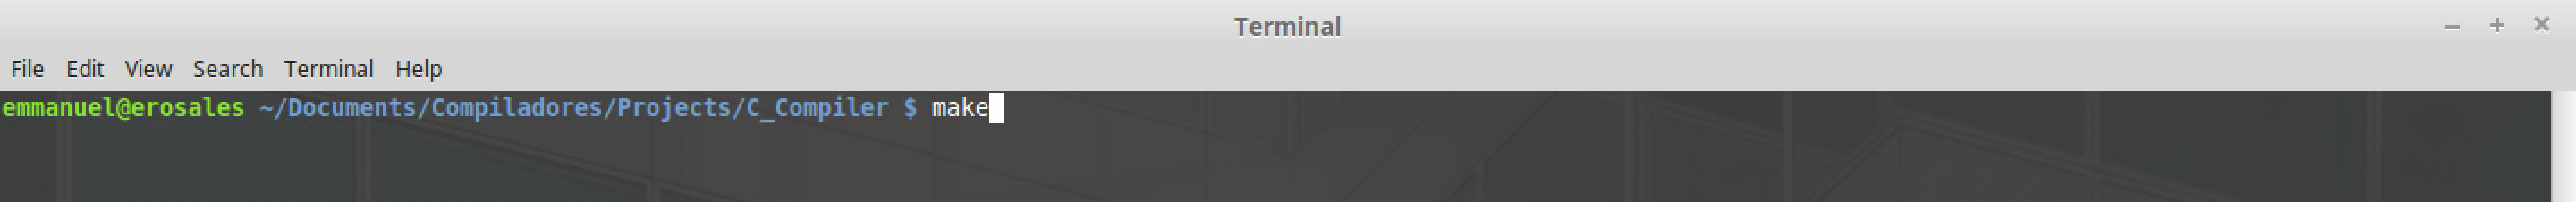
\includegraphics[height= 1.2cm]{main1}
    \end{center}

    
    Asimismo, una vez que el make es ejecutado correctamente, procedemos a llamar a la función main utilizando ./main + la dirección del archivo a compilar, este archivo debe tener extensión .micro
    
	\begin{center}
    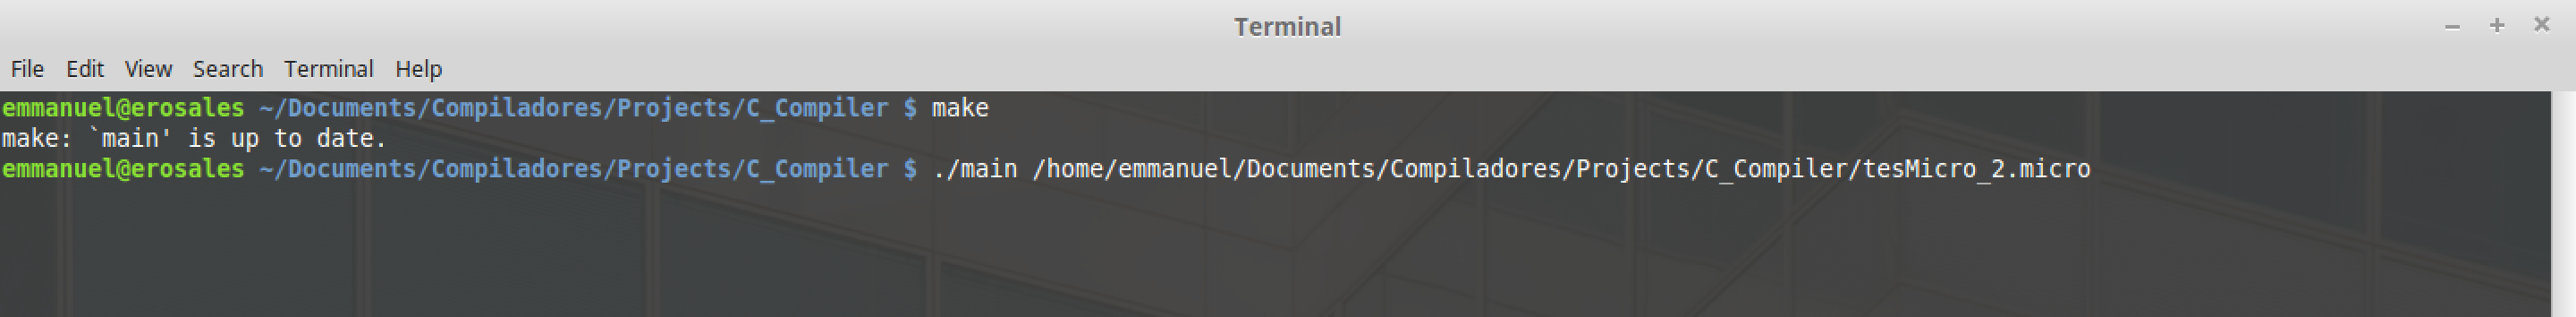
\includegraphics[height= 2cm]{main2}
    \end{center}
    
    Después de haber ejecutado la línea anterior, se mostrará en la terminal los tokens que fueron creados por el compilador.
    \begin{center}
    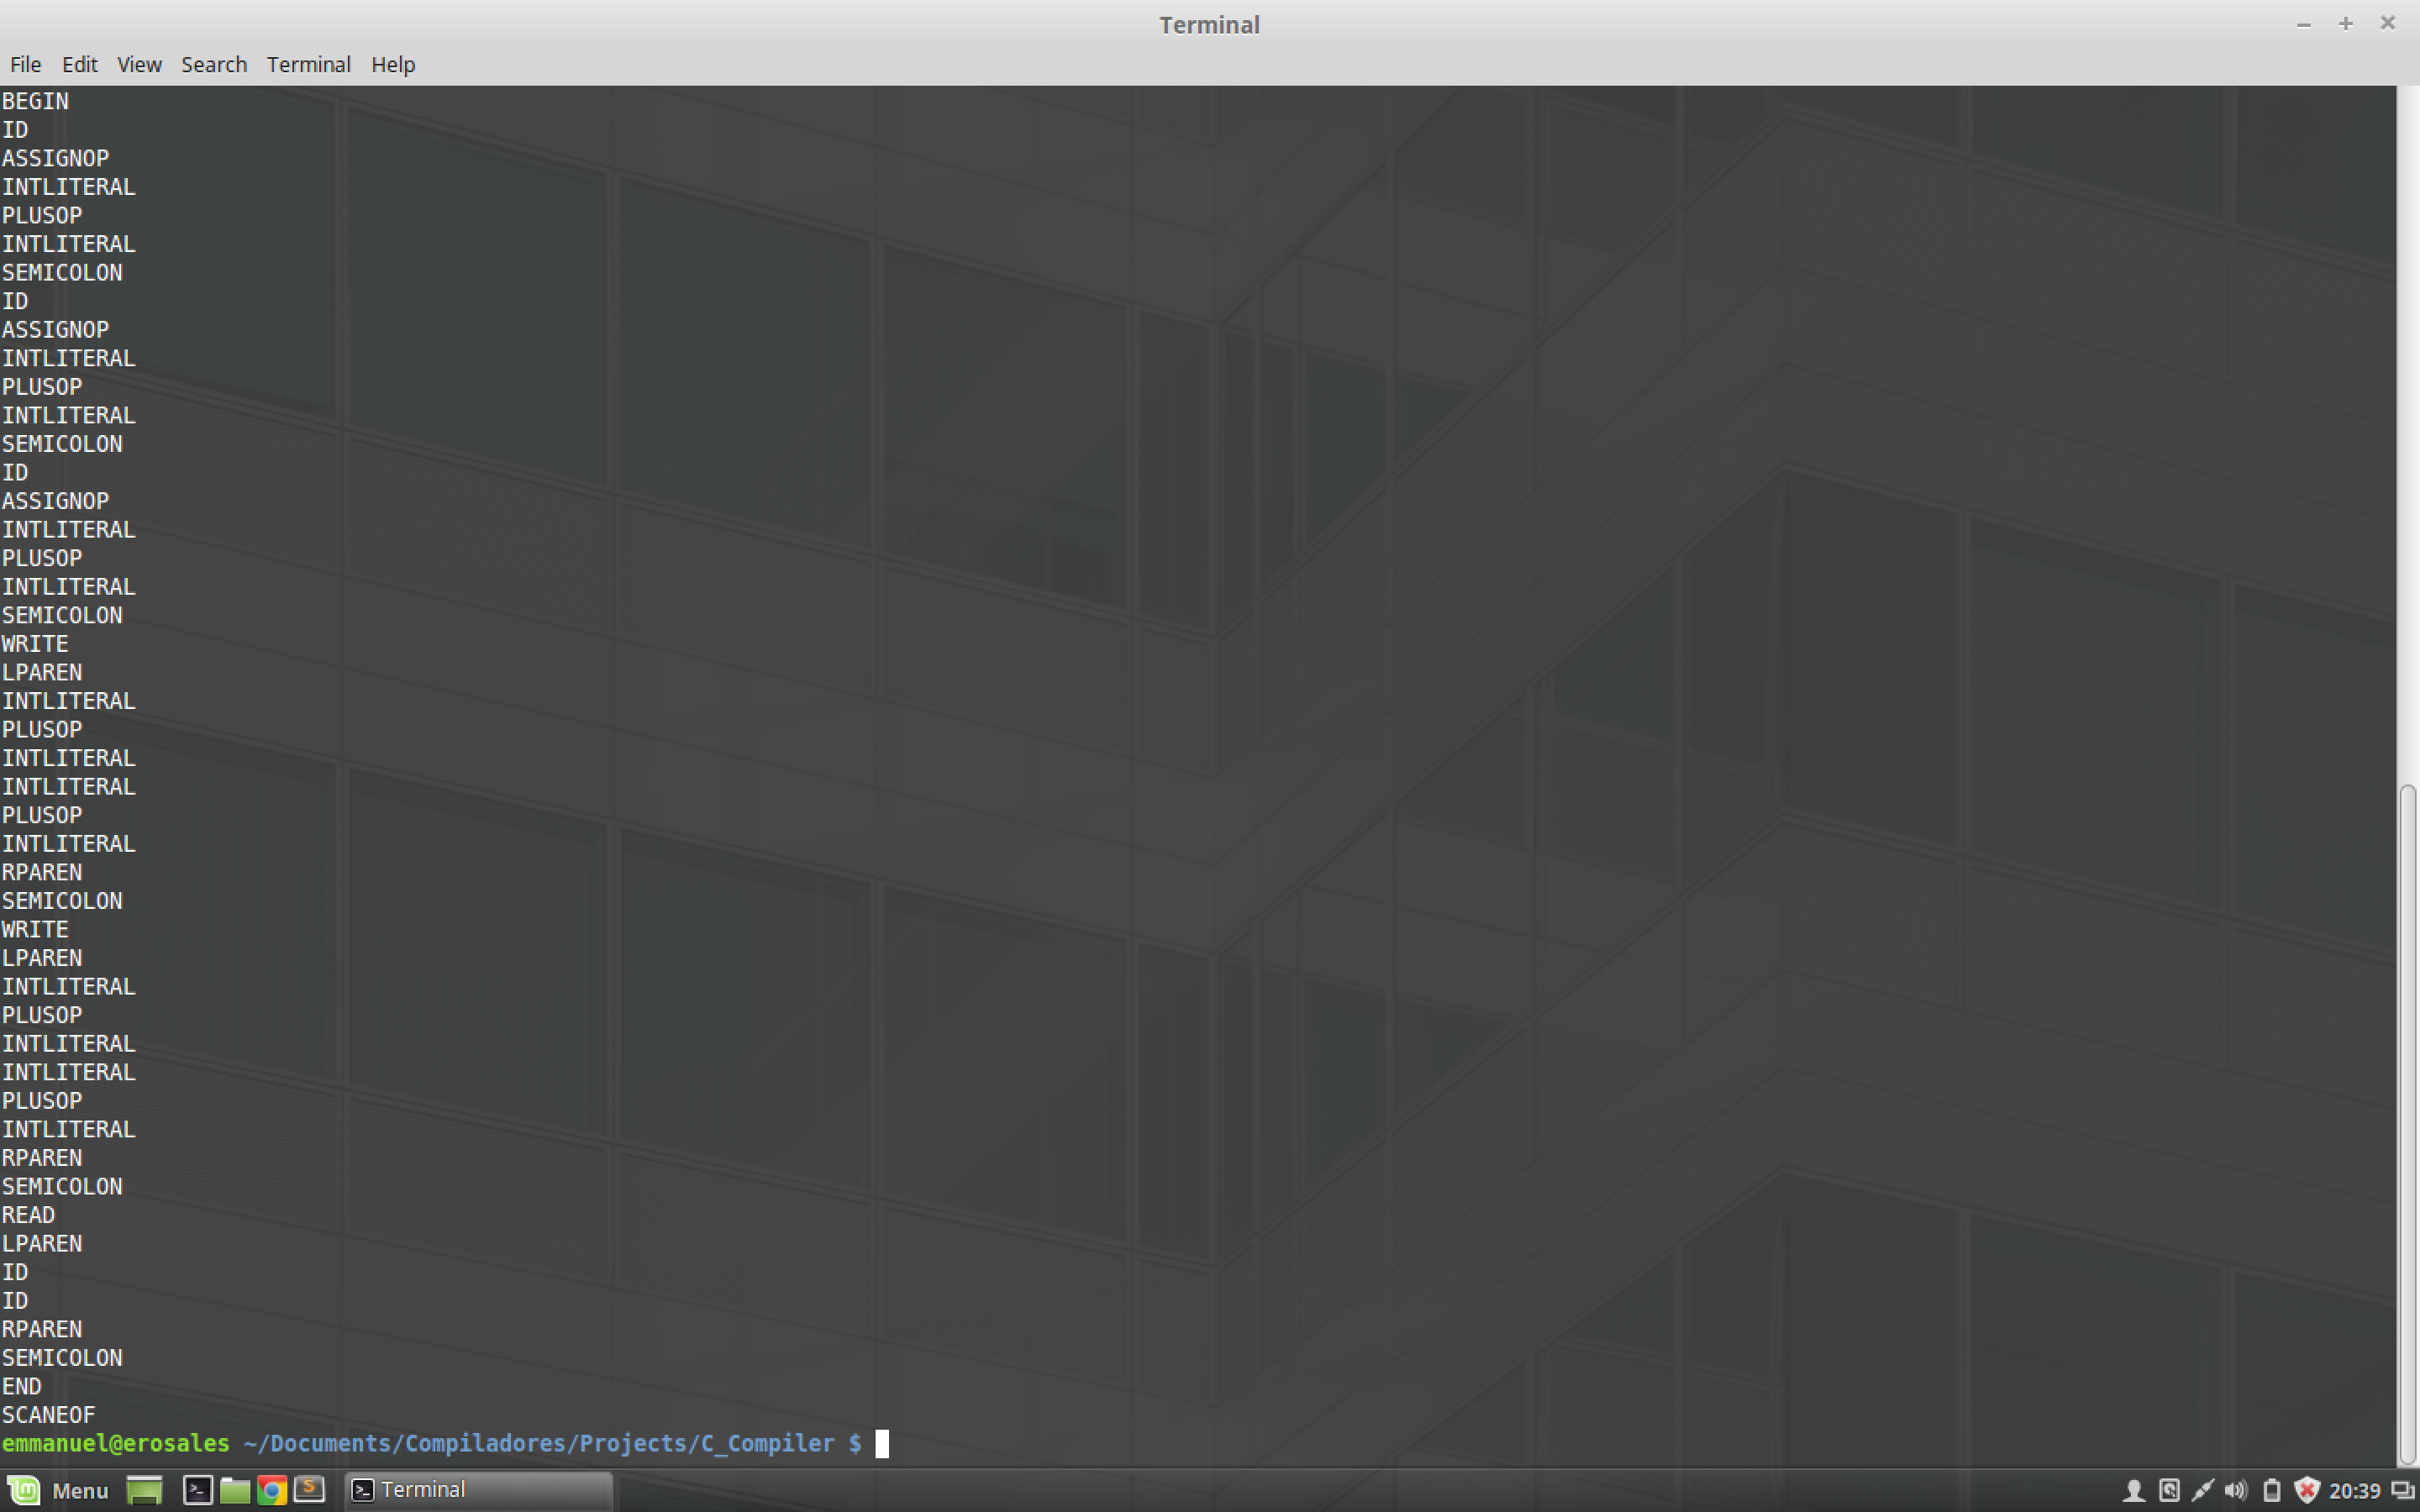
\includegraphics[height= 7cm]{main3}
    \end{center}

    Si el archivo fuente no tiene ningún error, y todo el proceso fue finalizado correctamente, en la ruta donde se encuentran los archivos del compilador se creo un archivo con el mismo nombre del archivo fuente pero con extensión .asm, ahí se podrá encontrar el código ensamblador de mips 
    \begin{center}
    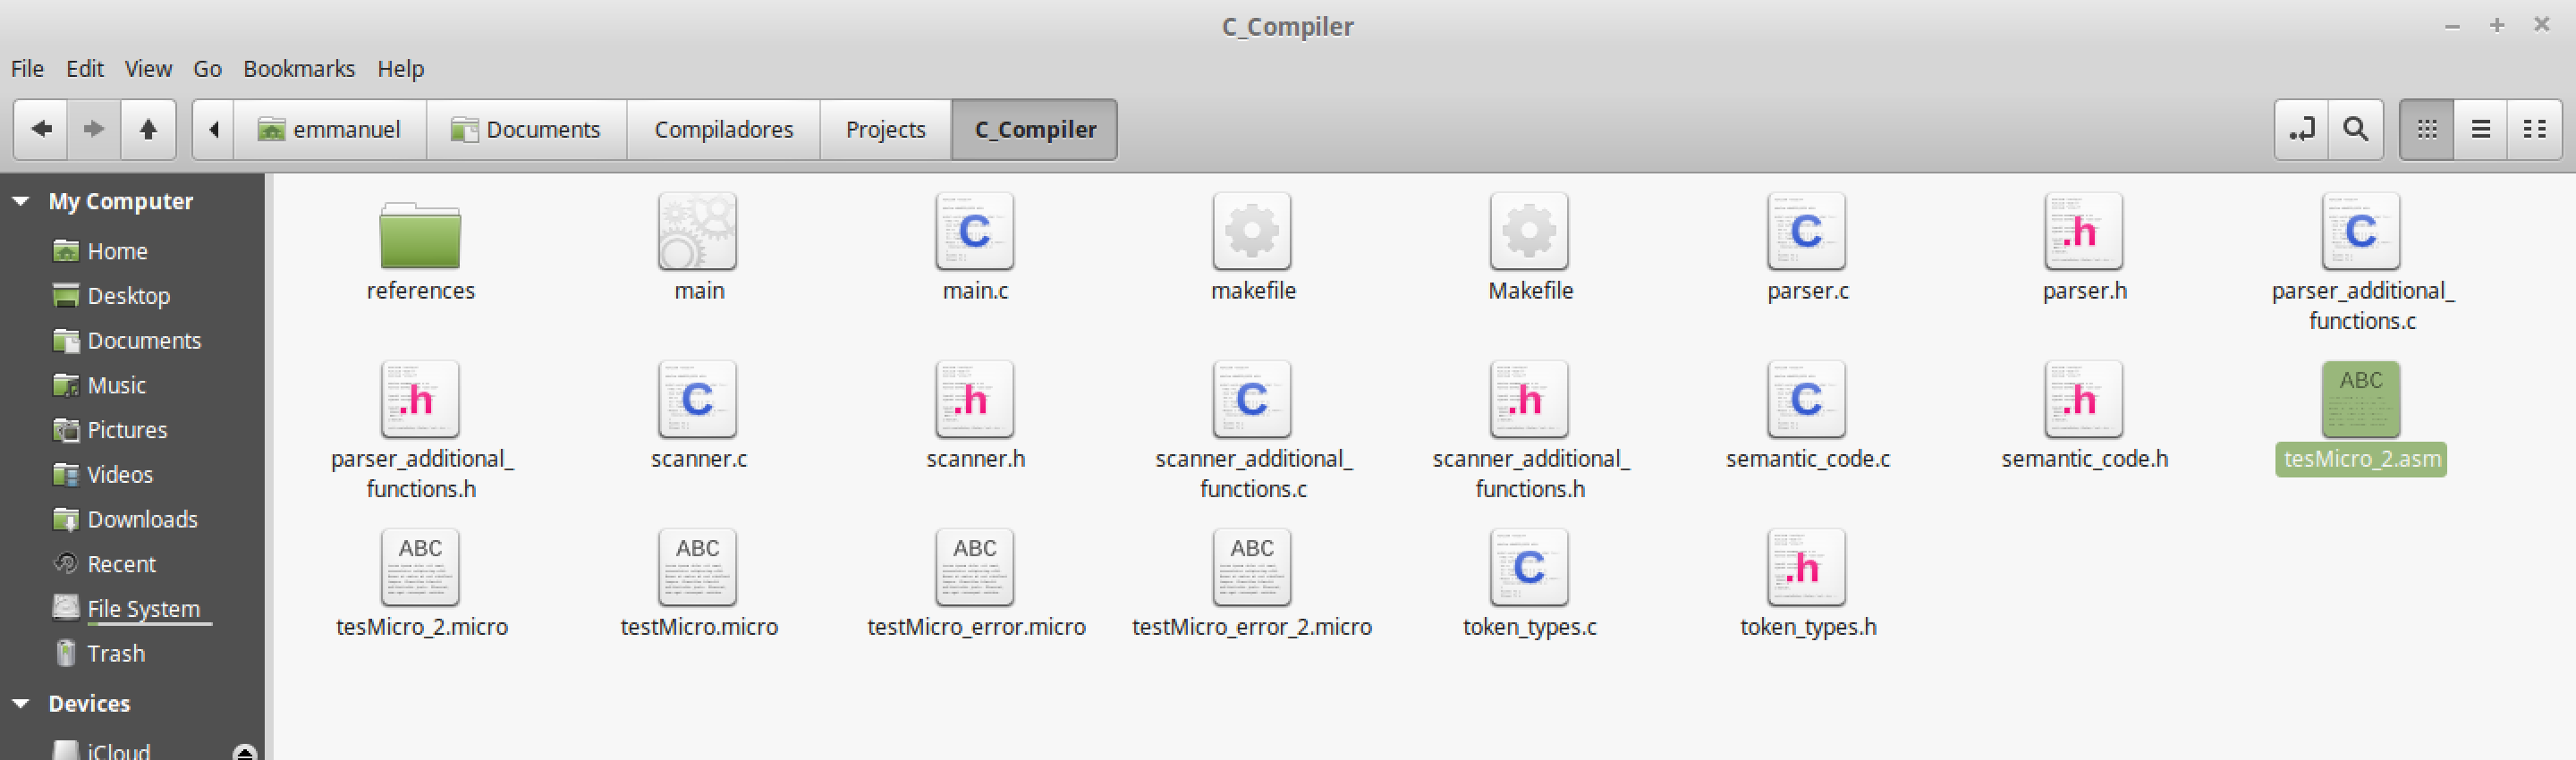
\includegraphics[height= 4cm]{main4}
    \end{center}
   
    Por ejemplo…
    
    \begin{center}
    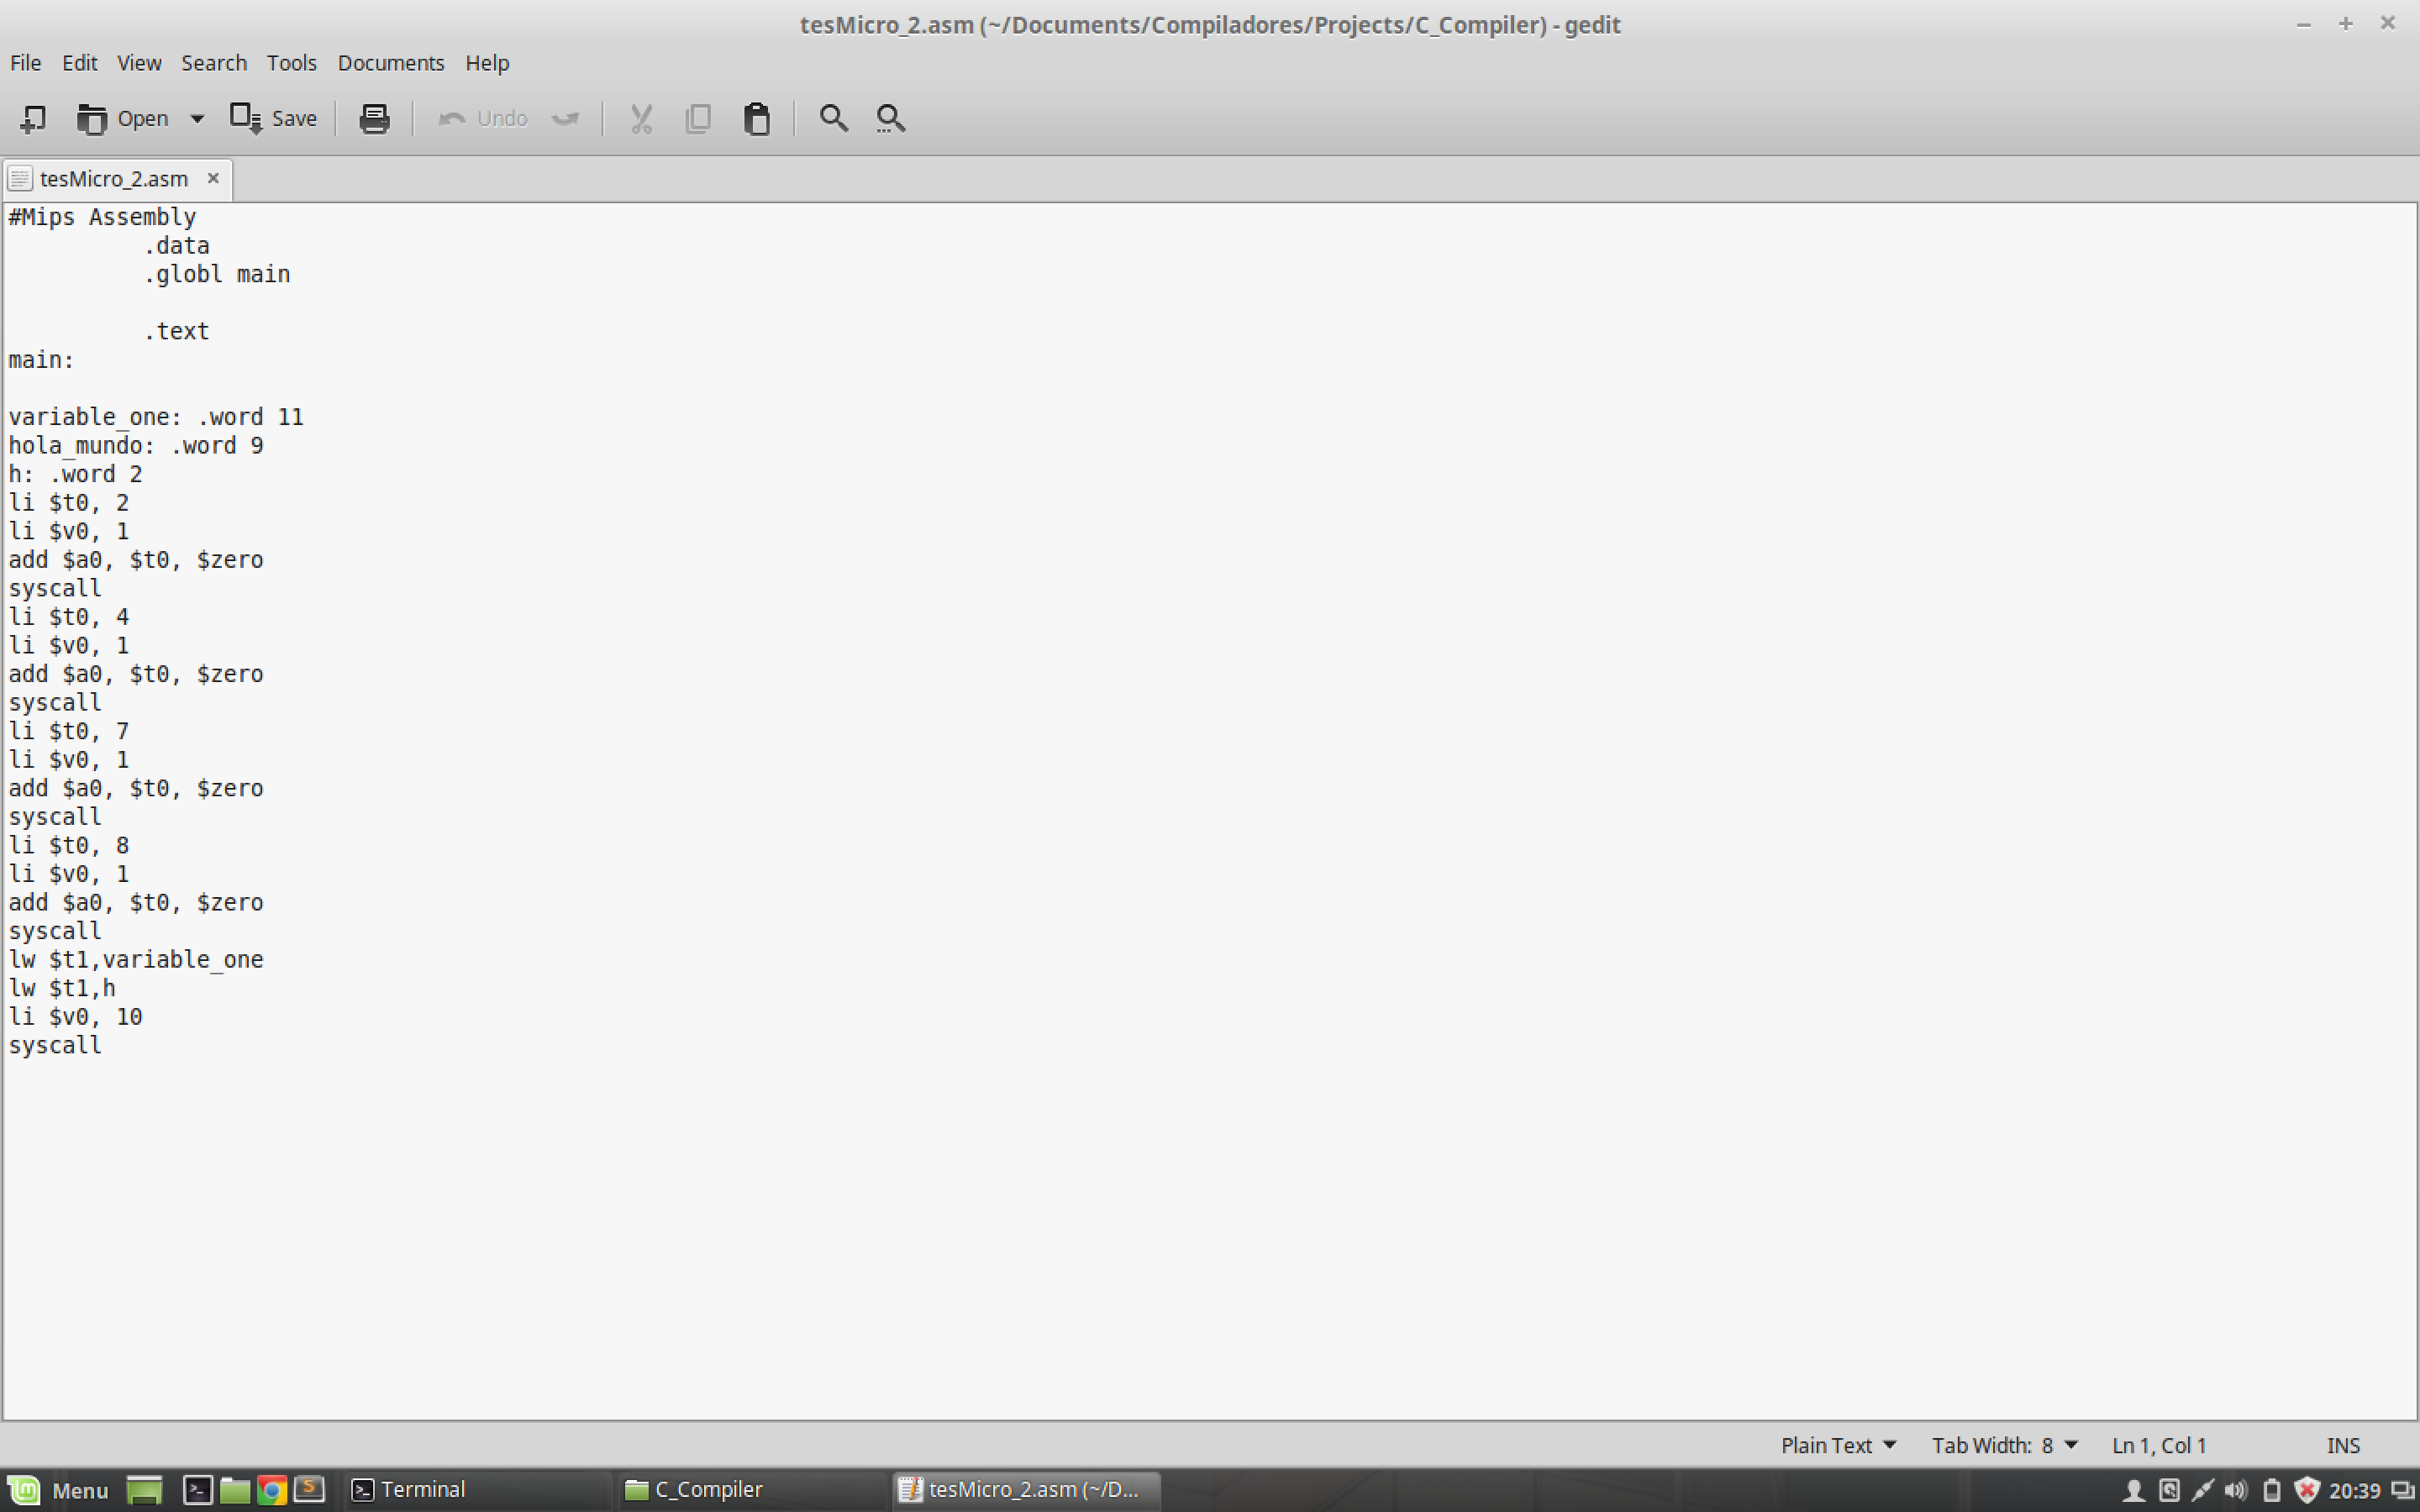
\includegraphics[height= 8cm]{main5}
    \end{center}
    

    Para poder probar si el compilador trabaja correctamente, es necesario usar un simulador de SPIM, este se puede descargar e instalar fácilmente, además es recomendable instalar su versión gráfica (qtspim) para una mayor facilidad para ejecutar las pruebas.
    Para iniciar el simulador, debemos ejecutar el comando qtspim para cargar el programa.
    
    \begin{center}
    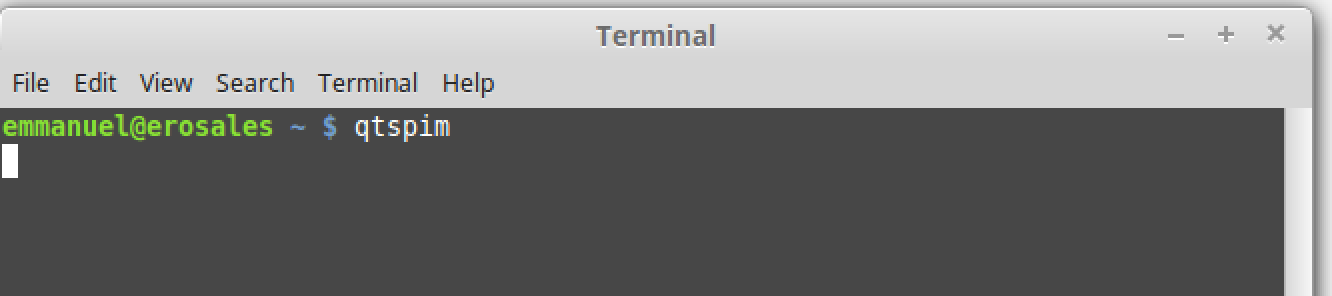
\includegraphics[height= 3cm]{main6}
    \end{center}

    La siguiente imagen muestra la pantalla principal del simulador de SPIM, para ejecutar nuestro archivo creado por el compilador debemos ir a File  Reinitialize and load file 
    
    \begin{center}
    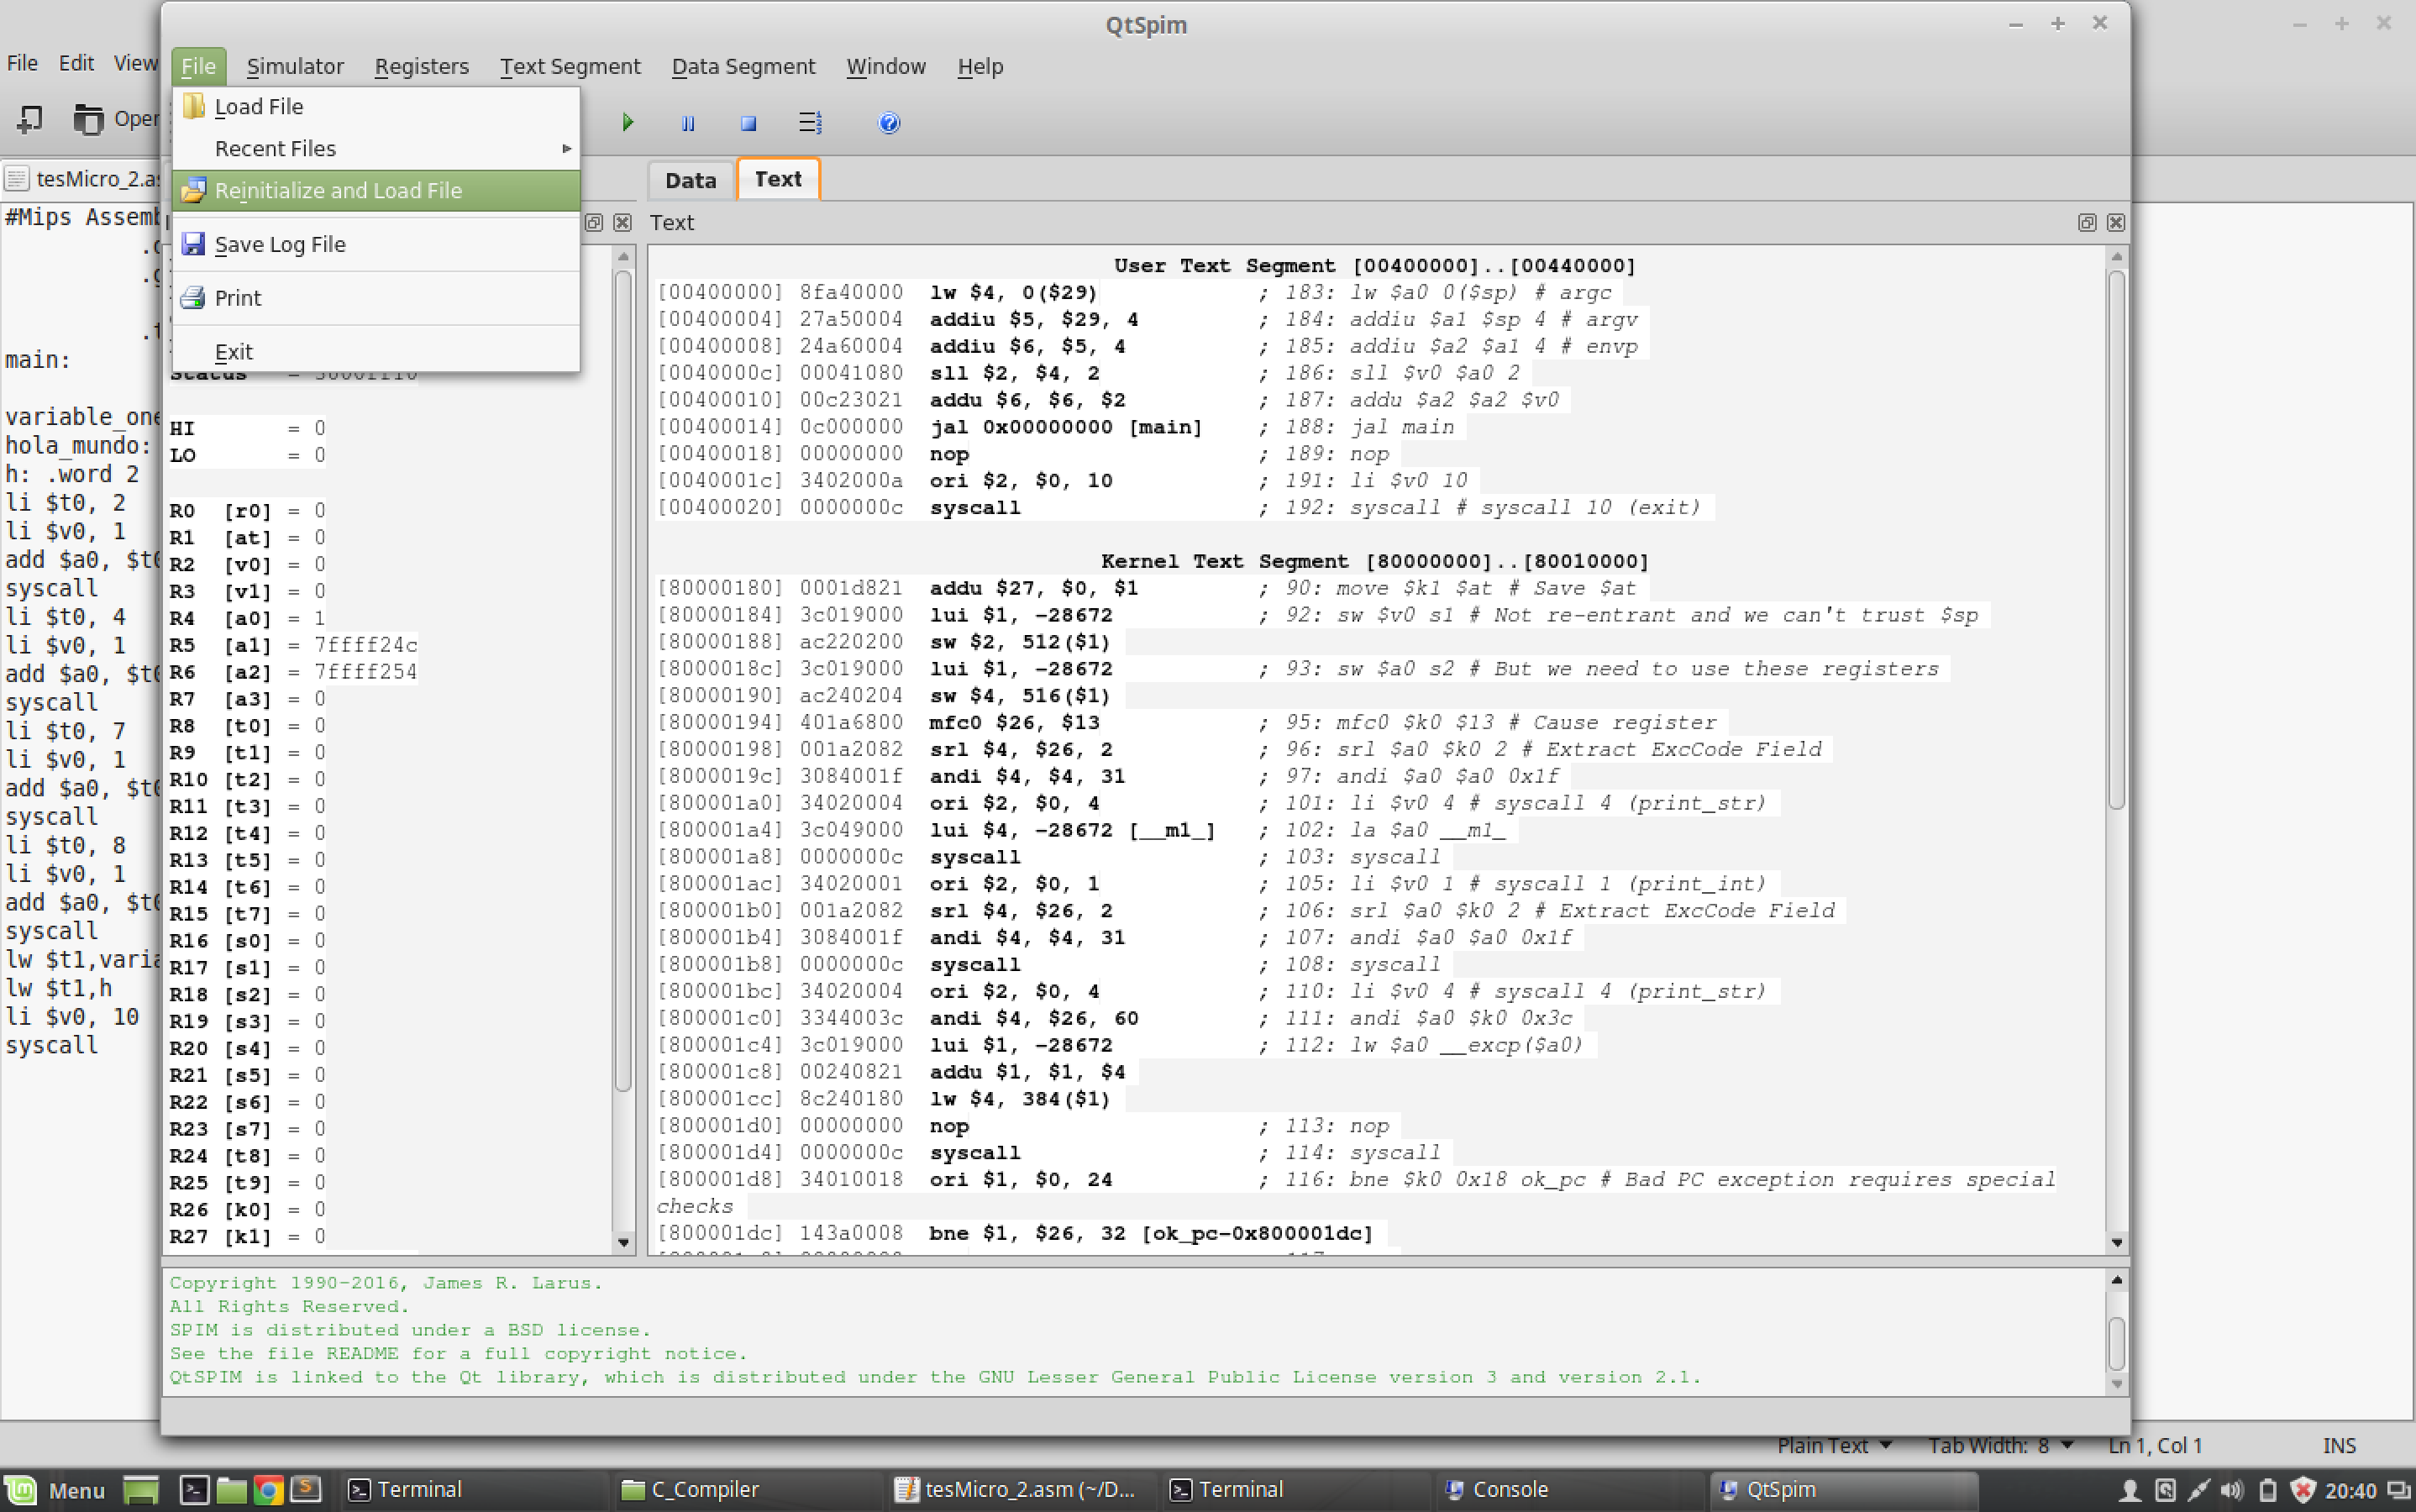
\includegraphics[height= 8cm]{main7}
    \end{center}

    y escogemos nuestro archivo.
\begin{center}
    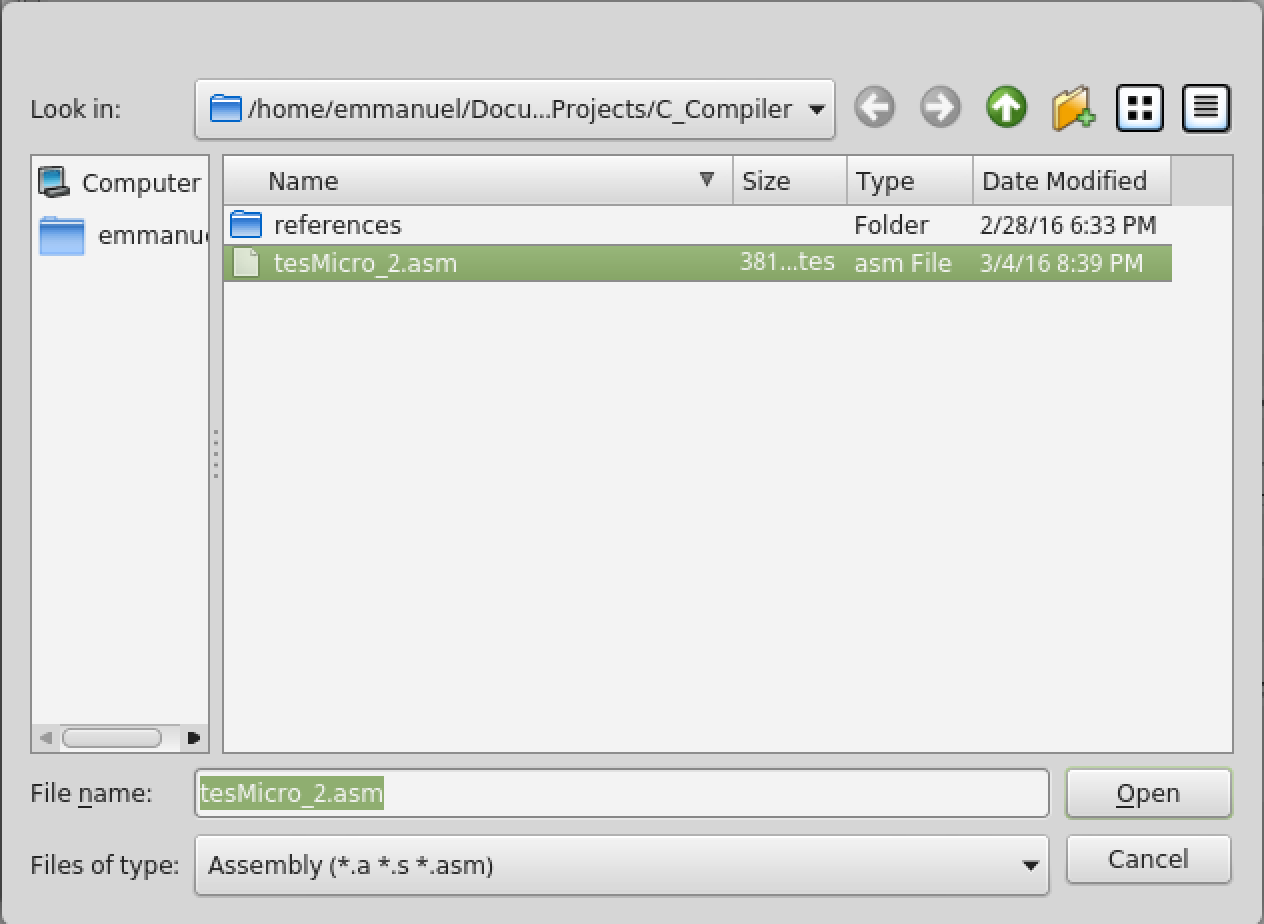
\includegraphics[height= 8cm]{main8}
    \end{center}

    Una vez cargado el archivo, podemos procederlo a ejecutar y en la consola va a mostrar los resultados.

\begin{center}
    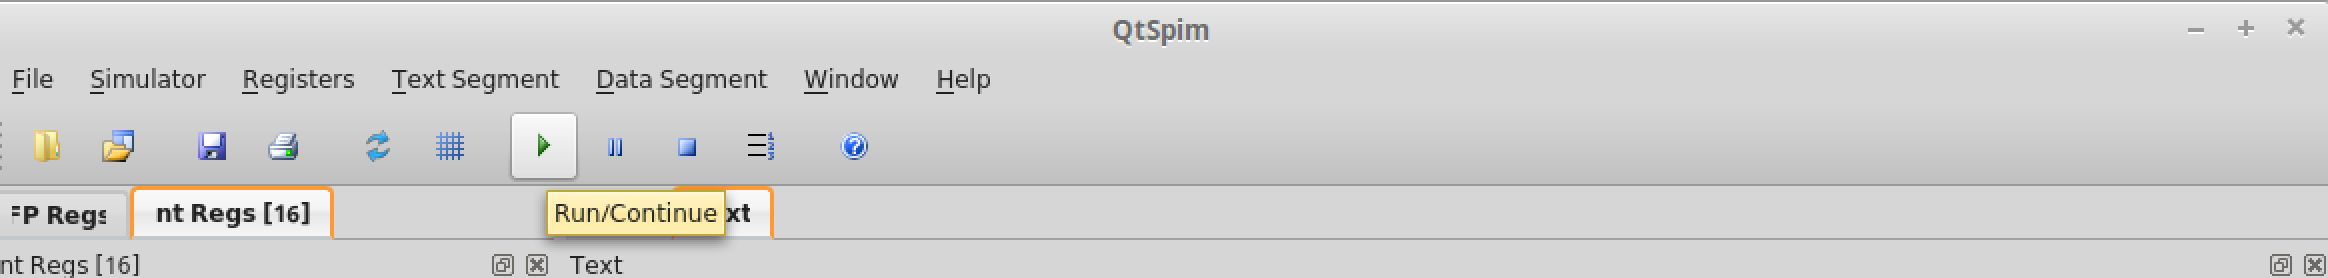
\includegraphics[height= 2cm]{main9}
    \end{center}


\end{document}
